% Created by tikzDevice version 0.12.6 on 2024-03-06 16:34:20
% !TEX encoding = UTF-8 Unicode
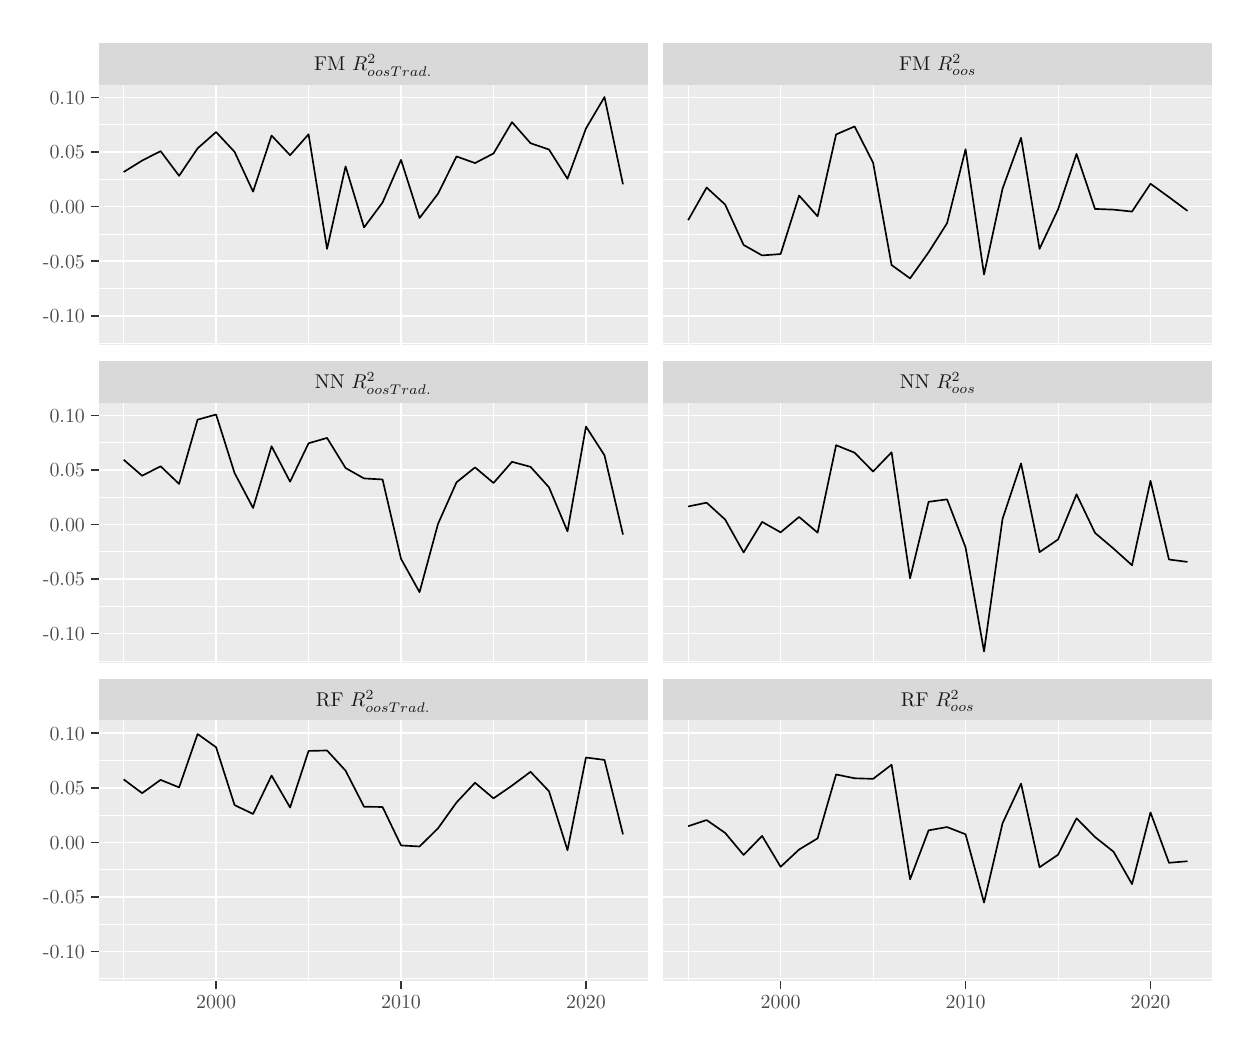
\begin{tikzpicture}[x=1pt,y=1pt]
\definecolor{fillColor}{RGB}{255,255,255}
\path[use as bounding box,fill=fillColor,fill opacity=0.00] (0,0) rectangle (433.62,361.35);
\begin{scope}
\path[clip] (  0.00,  0.00) rectangle (433.62,361.35);
\definecolor{drawColor}{RGB}{255,255,255}
\definecolor{fillColor}{RGB}{255,255,255}

\path[draw=drawColor,line width= 0.6pt,line join=round,line cap=round,fill=fillColor] (  0.00,  0.00) rectangle (433.62,361.35);
\end{scope}
\begin{scope}
\path[clip] ( 25.65,246.50) rectangle (224.13,340.69);
\definecolor{fillColor}{gray}{0.92}

\path[fill=fillColor] ( 25.65,246.50) rectangle (224.13,340.69);
\definecolor{drawColor}{RGB}{255,255,255}

\path[draw=drawColor,line width= 0.3pt,line join=round] ( 25.65,247.37) --
	(224.13,247.37);

\path[draw=drawColor,line width= 0.3pt,line join=round] ( 25.65,267.09) --
	(224.13,267.09);

\path[draw=drawColor,line width= 0.3pt,line join=round] ( 25.65,286.81) --
	(224.13,286.81);

\path[draw=drawColor,line width= 0.3pt,line join=round] ( 25.65,306.53) --
	(224.13,306.53);

\path[draw=drawColor,line width= 0.3pt,line join=round] ( 25.65,326.25) --
	(224.13,326.25);

\path[draw=drawColor,line width= 0.3pt,line join=round] ( 34.67,246.50) --
	( 34.67,340.69);

\path[draw=drawColor,line width= 0.3pt,line join=round] (101.50,246.50) --
	(101.50,340.69);

\path[draw=drawColor,line width= 0.3pt,line join=round] (168.33,246.50) --
	(168.33,340.69);

\path[draw=drawColor,line width= 0.6pt,line join=round] ( 25.65,257.23) --
	(224.13,257.23);

\path[draw=drawColor,line width= 0.6pt,line join=round] ( 25.65,276.95) --
	(224.13,276.95);

\path[draw=drawColor,line width= 0.6pt,line join=round] ( 25.65,296.67) --
	(224.13,296.67);

\path[draw=drawColor,line width= 0.6pt,line join=round] ( 25.65,316.39) --
	(224.13,316.39);

\path[draw=drawColor,line width= 0.6pt,line join=round] ( 25.65,336.11) --
	(224.13,336.11);

\path[draw=drawColor,line width= 0.6pt,line join=round] ( 68.08,246.50) --
	( 68.08,340.69);

\path[draw=drawColor,line width= 0.6pt,line join=round] (134.91,246.50) --
	(134.91,340.69);

\path[draw=drawColor,line width= 0.6pt,line join=round] (201.74,246.50) --
	(201.74,340.69);
\definecolor{drawColor}{RGB}{0,0,0}

\path[draw=drawColor,line width= 0.6pt,line join=round] ( 34.67,309.18) --
	( 41.35,313.32) --
	( 48.03,316.73) --
	( 54.72,307.81) --
	( 61.40,317.73) --
	( 68.08,323.64) --
	( 74.77,316.46) --
	( 81.45,302.09) --
	( 88.13,322.37) --
	( 94.82,315.26) --
	(101.50,322.82) --
	(108.18,281.42) --
	(114.87,311.22) --
	(121.55,289.17) --
	(128.23,298.16) --
	(134.91,313.58) --
	(141.60,292.56) --
	(148.28,301.35) --
	(154.96,314.81) --
	(161.65,312.42) --
	(168.33,315.89) --
	(175.01,327.21) --
	(181.70,319.60) --
	(188.38,317.32) --
	(195.06,306.75) --
	(201.74,324.93) --
	(208.43,336.27) --
	(215.11,304.74);
\end{scope}
\begin{scope}
\path[clip] ( 25.65,131.66) rectangle (224.13,225.84);
\definecolor{fillColor}{gray}{0.92}

\path[fill=fillColor] ( 25.65,131.66) rectangle (224.13,225.84);
\definecolor{drawColor}{RGB}{255,255,255}

\path[draw=drawColor,line width= 0.3pt,line join=round] ( 25.65,132.52) --
	(224.13,132.52);

\path[draw=drawColor,line width= 0.3pt,line join=round] ( 25.65,152.24) --
	(224.13,152.24);

\path[draw=drawColor,line width= 0.3pt,line join=round] ( 25.65,171.96) --
	(224.13,171.96);

\path[draw=drawColor,line width= 0.3pt,line join=round] ( 25.65,191.68) --
	(224.13,191.68);

\path[draw=drawColor,line width= 0.3pt,line join=round] ( 25.65,211.40) --
	(224.13,211.40);

\path[draw=drawColor,line width= 0.3pt,line join=round] ( 34.67,131.66) --
	( 34.67,225.84);

\path[draw=drawColor,line width= 0.3pt,line join=round] (101.50,131.66) --
	(101.50,225.84);

\path[draw=drawColor,line width= 0.3pt,line join=round] (168.33,131.66) --
	(168.33,225.84);

\path[draw=drawColor,line width= 0.6pt,line join=round] ( 25.65,142.38) --
	(224.13,142.38);

\path[draw=drawColor,line width= 0.6pt,line join=round] ( 25.65,162.10) --
	(224.13,162.10);

\path[draw=drawColor,line width= 0.6pt,line join=round] ( 25.65,181.82) --
	(224.13,181.82);

\path[draw=drawColor,line width= 0.6pt,line join=round] ( 25.65,201.54) --
	(224.13,201.54);

\path[draw=drawColor,line width= 0.6pt,line join=round] ( 25.65,221.26) --
	(224.13,221.26);

\path[draw=drawColor,line width= 0.6pt,line join=round] ( 68.08,131.66) --
	( 68.08,225.84);

\path[draw=drawColor,line width= 0.6pt,line join=round] (134.91,131.66) --
	(134.91,225.84);

\path[draw=drawColor,line width= 0.6pt,line join=round] (201.74,131.66) --
	(201.74,225.84);
\definecolor{drawColor}{RGB}{0,0,0}

\path[draw=drawColor,line width= 0.6pt,line join=round] ( 34.67,205.23) --
	( 41.35,199.43) --
	( 48.03,202.86) --
	( 54.72,196.48) --
	( 61.40,219.70) --
	( 68.08,221.56) --
	( 74.77,200.39) --
	( 81.45,187.78) --
	( 88.13,210.08) --
	( 94.82,197.29) --
	(101.50,211.17) --
	(108.18,213.10) --
	(114.87,202.23) --
	(121.55,198.46) --
	(128.23,198.09) --
	(134.91,169.42) --
	(141.60,157.36) --
	(148.28,182.05) --
	(154.96,197.06) --
	(161.65,202.45) --
	(168.33,196.82) --
	(175.01,204.47) --
	(181.70,202.66) --
	(188.38,195.25) --
	(195.06,179.34) --
	(201.74,217.21) --
	(208.43,206.82) --
	(215.11,178.18);
\end{scope}
\begin{scope}
\path[clip] ( 25.65, 16.81) rectangle (224.13,111.00);
\definecolor{fillColor}{gray}{0.92}

\path[fill=fillColor] ( 25.65, 16.81) rectangle (224.13,111.00);
\definecolor{drawColor}{RGB}{255,255,255}

\path[draw=drawColor,line width= 0.3pt,line join=round] ( 25.65, 17.67) --
	(224.13, 17.67);

\path[draw=drawColor,line width= 0.3pt,line join=round] ( 25.65, 37.39) --
	(224.13, 37.39);

\path[draw=drawColor,line width= 0.3pt,line join=round] ( 25.65, 57.11) --
	(224.13, 57.11);

\path[draw=drawColor,line width= 0.3pt,line join=round] ( 25.65, 76.83) --
	(224.13, 76.83);

\path[draw=drawColor,line width= 0.3pt,line join=round] ( 25.65, 96.56) --
	(224.13, 96.56);

\path[draw=drawColor,line width= 0.3pt,line join=round] ( 34.67, 16.81) --
	( 34.67,111.00);

\path[draw=drawColor,line width= 0.3pt,line join=round] (101.50, 16.81) --
	(101.50,111.00);

\path[draw=drawColor,line width= 0.3pt,line join=round] (168.33, 16.81) --
	(168.33,111.00);

\path[draw=drawColor,line width= 0.6pt,line join=round] ( 25.65, 27.53) --
	(224.13, 27.53);

\path[draw=drawColor,line width= 0.6pt,line join=round] ( 25.65, 47.25) --
	(224.13, 47.25);

\path[draw=drawColor,line width= 0.6pt,line join=round] ( 25.65, 66.97) --
	(224.13, 66.97);

\path[draw=drawColor,line width= 0.6pt,line join=round] ( 25.65, 86.69) --
	(224.13, 86.69);

\path[draw=drawColor,line width= 0.6pt,line join=round] ( 25.65,106.42) --
	(224.13,106.42);

\path[draw=drawColor,line width= 0.6pt,line join=round] ( 68.08, 16.81) --
	( 68.08,111.00);

\path[draw=drawColor,line width= 0.6pt,line join=round] (134.91, 16.81) --
	(134.91,111.00);

\path[draw=drawColor,line width= 0.6pt,line join=round] (201.74, 16.81) --
	(201.74,111.00);
\definecolor{drawColor}{RGB}{0,0,0}

\path[draw=drawColor,line width= 0.6pt,line join=round] ( 34.67, 89.72) --
	( 41.35, 84.74) --
	( 48.03, 89.54) --
	( 54.72, 86.82) --
	( 61.40,106.10) --
	( 68.08,101.34) --
	( 74.77, 80.42) --
	( 81.45, 77.22) --
	( 88.13, 91.10) --
	( 94.82, 79.56) --
	(101.50,100.00) --
	(108.18,100.16) --
	(114.87, 92.87) --
	(121.55, 79.83) --
	(128.23, 79.75) --
	(134.91, 65.85) --
	(141.60, 65.47) --
	(148.28, 72.04) --
	(154.96, 81.38) --
	(161.65, 88.50) --
	(168.33, 82.87) --
	(175.01, 87.46) --
	(181.70, 92.46) --
	(188.38, 85.43) --
	(195.06, 64.12) --
	(201.74, 97.62) --
	(208.43, 96.75) --
	(215.11, 69.86);
\end{scope}
\begin{scope}
\path[clip] (229.63,246.50) rectangle (428.12,340.69);
\definecolor{fillColor}{gray}{0.92}

\path[fill=fillColor] (229.63,246.50) rectangle (428.12,340.69);
\definecolor{drawColor}{RGB}{255,255,255}

\path[draw=drawColor,line width= 0.3pt,line join=round] (229.63,247.37) --
	(428.12,247.37);

\path[draw=drawColor,line width= 0.3pt,line join=round] (229.63,267.09) --
	(428.12,267.09);

\path[draw=drawColor,line width= 0.3pt,line join=round] (229.63,286.81) --
	(428.12,286.81);

\path[draw=drawColor,line width= 0.3pt,line join=round] (229.63,306.53) --
	(428.12,306.53);

\path[draw=drawColor,line width= 0.3pt,line join=round] (229.63,326.25) --
	(428.12,326.25);

\path[draw=drawColor,line width= 0.3pt,line join=round] (238.66,246.50) --
	(238.66,340.69);

\path[draw=drawColor,line width= 0.3pt,line join=round] (305.49,246.50) --
	(305.49,340.69);

\path[draw=drawColor,line width= 0.3pt,line join=round] (372.32,246.50) --
	(372.32,340.69);

\path[draw=drawColor,line width= 0.6pt,line join=round] (229.63,257.23) --
	(428.12,257.23);

\path[draw=drawColor,line width= 0.6pt,line join=round] (229.63,276.95) --
	(428.12,276.95);

\path[draw=drawColor,line width= 0.6pt,line join=round] (229.63,296.67) --
	(428.12,296.67);

\path[draw=drawColor,line width= 0.6pt,line join=round] (229.63,316.39) --
	(428.12,316.39);

\path[draw=drawColor,line width= 0.6pt,line join=round] (229.63,336.11) --
	(428.12,336.11);

\path[draw=drawColor,line width= 0.6pt,line join=round] (272.07,246.50) --
	(272.07,340.69);

\path[draw=drawColor,line width= 0.6pt,line join=round] (338.90,246.50) --
	(338.90,340.69);

\path[draw=drawColor,line width= 0.6pt,line join=round] (405.73,246.50) --
	(405.73,340.69);
\definecolor{drawColor}{RGB}{0,0,0}

\path[draw=drawColor,line width= 0.6pt,line join=round] (238.66,291.79) --
	(245.34,303.57) --
	(252.02,297.44) --
	(258.70,282.83) --
	(265.39,279.05) --
	(272.07,279.54) --
	(278.75,300.68) --
	(285.44,293.17) --
	(292.12,322.76) --
	(298.80,325.66) --
	(305.49,312.54) --
	(312.17,275.57) --
	(318.85,270.75) --
	(325.54,280.18) --
	(332.22,290.69) --
	(338.90,317.43) --
	(345.58,272.18) --
	(352.27,303.17) --
	(358.95,321.57) --
	(365.63,281.41) --
	(372.32,295.70) --
	(379.00,315.72) --
	(385.68,295.85) --
	(392.37,295.60) --
	(399.05,294.89) --
	(405.73,304.95) --
	(412.41,300.11) --
	(419.10,295.14);
\end{scope}
\begin{scope}
\path[clip] (229.63,131.66) rectangle (428.12,225.84);
\definecolor{fillColor}{gray}{0.92}

\path[fill=fillColor] (229.63,131.66) rectangle (428.12,225.84);
\definecolor{drawColor}{RGB}{255,255,255}

\path[draw=drawColor,line width= 0.3pt,line join=round] (229.63,132.52) --
	(428.12,132.52);

\path[draw=drawColor,line width= 0.3pt,line join=round] (229.63,152.24) --
	(428.12,152.24);

\path[draw=drawColor,line width= 0.3pt,line join=round] (229.63,171.96) --
	(428.12,171.96);

\path[draw=drawColor,line width= 0.3pt,line join=round] (229.63,191.68) --
	(428.12,191.68);

\path[draw=drawColor,line width= 0.3pt,line join=round] (229.63,211.40) --
	(428.12,211.40);

\path[draw=drawColor,line width= 0.3pt,line join=round] (238.66,131.66) --
	(238.66,225.84);

\path[draw=drawColor,line width= 0.3pt,line join=round] (305.49,131.66) --
	(305.49,225.84);

\path[draw=drawColor,line width= 0.3pt,line join=round] (372.32,131.66) --
	(372.32,225.84);

\path[draw=drawColor,line width= 0.6pt,line join=round] (229.63,142.38) --
	(428.12,142.38);

\path[draw=drawColor,line width= 0.6pt,line join=round] (229.63,162.10) --
	(428.12,162.10);

\path[draw=drawColor,line width= 0.6pt,line join=round] (229.63,181.82) --
	(428.12,181.82);

\path[draw=drawColor,line width= 0.6pt,line join=round] (229.63,201.54) --
	(428.12,201.54);

\path[draw=drawColor,line width= 0.6pt,line join=round] (229.63,221.26) --
	(428.12,221.26);

\path[draw=drawColor,line width= 0.6pt,line join=round] (272.07,131.66) --
	(272.07,225.84);

\path[draw=drawColor,line width= 0.6pt,line join=round] (338.90,131.66) --
	(338.90,225.84);

\path[draw=drawColor,line width= 0.6pt,line join=round] (405.73,131.66) --
	(405.73,225.84);
\definecolor{drawColor}{RGB}{0,0,0}

\path[draw=drawColor,line width= 0.6pt,line join=round] (238.66,188.33) --
	(245.34,189.70) --
	(252.02,183.63) --
	(258.70,171.73) --
	(265.39,182.76) --
	(272.07,178.99) --
	(278.75,184.55) --
	(285.44,178.87) --
	(292.12,210.47) --
	(298.80,207.77) --
	(305.49,200.97) --
	(312.17,207.91) --
	(318.85,162.38) --
	(325.54,190.01) --
	(332.22,190.90) --
	(338.90,173.56) --
	(345.58,135.94) --
	(352.27,183.89) --
	(358.95,203.87) --
	(365.63,171.84) --
	(372.32,176.40) --
	(379.00,192.73) --
	(385.68,178.78) --
	(392.37,173.11) --
	(399.05,167.10) --
	(405.73,197.62) --
	(412.41,169.17) --
	(419.10,168.30);
\end{scope}
\begin{scope}
\path[clip] (229.63, 16.81) rectangle (428.12,111.00);
\definecolor{fillColor}{gray}{0.92}

\path[fill=fillColor] (229.63, 16.81) rectangle (428.12,111.00);
\definecolor{drawColor}{RGB}{255,255,255}

\path[draw=drawColor,line width= 0.3pt,line join=round] (229.63, 17.67) --
	(428.12, 17.67);

\path[draw=drawColor,line width= 0.3pt,line join=round] (229.63, 37.39) --
	(428.12, 37.39);

\path[draw=drawColor,line width= 0.3pt,line join=round] (229.63, 57.11) --
	(428.12, 57.11);

\path[draw=drawColor,line width= 0.3pt,line join=round] (229.63, 76.83) --
	(428.12, 76.83);

\path[draw=drawColor,line width= 0.3pt,line join=round] (229.63, 96.56) --
	(428.12, 96.56);

\path[draw=drawColor,line width= 0.3pt,line join=round] (238.66, 16.81) --
	(238.66,111.00);

\path[draw=drawColor,line width= 0.3pt,line join=round] (305.49, 16.81) --
	(305.49,111.00);

\path[draw=drawColor,line width= 0.3pt,line join=round] (372.32, 16.81) --
	(372.32,111.00);

\path[draw=drawColor,line width= 0.6pt,line join=round] (229.63, 27.53) --
	(428.12, 27.53);

\path[draw=drawColor,line width= 0.6pt,line join=round] (229.63, 47.25) --
	(428.12, 47.25);

\path[draw=drawColor,line width= 0.6pt,line join=round] (229.63, 66.97) --
	(428.12, 66.97);

\path[draw=drawColor,line width= 0.6pt,line join=round] (229.63, 86.69) --
	(428.12, 86.69);

\path[draw=drawColor,line width= 0.6pt,line join=round] (229.63,106.42) --
	(428.12,106.42);

\path[draw=drawColor,line width= 0.6pt,line join=round] (272.07, 16.81) --
	(272.07,111.00);

\path[draw=drawColor,line width= 0.6pt,line join=round] (338.90, 16.81) --
	(338.90,111.00);

\path[draw=drawColor,line width= 0.6pt,line join=round] (405.73, 16.81) --
	(405.73,111.00);
\definecolor{drawColor}{RGB}{0,0,0}

\path[draw=drawColor,line width= 0.6pt,line join=round] (238.66, 72.80) --
	(245.34, 75.02) --
	(252.02, 70.38) --
	(258.70, 62.41) --
	(265.39, 69.29) --
	(272.07, 58.12) --
	(278.75, 64.37) --
	(285.44, 68.41) --
	(292.12, 91.49) --
	(298.80, 90.12) --
	(305.49, 89.91) --
	(312.17, 95.00) --
	(318.85, 53.60) --
	(325.54, 71.30) --
	(332.22, 72.49) --
	(338.90, 69.88) --
	(345.58, 45.21) --
	(352.27, 73.86) --
	(358.95, 88.20) --
	(365.63, 57.96) --
	(372.32, 62.49) --
	(379.00, 75.65) --
	(385.68, 68.89) --
	(392.37, 63.58) --
	(399.05, 51.87) --
	(405.73, 77.77) --
	(412.41, 59.58) --
	(419.10, 60.14);
\end{scope}
\begin{scope}
\path[clip] ( 25.65,111.00) rectangle (224.13,126.16);
\definecolor{fillColor}{gray}{0.85}

\path[fill=fillColor] ( 25.65,111.00) rectangle (224.13,126.16);
\definecolor{drawColor}{gray}{0.10}

\node[text=drawColor,anchor=base,inner sep=0pt, outer sep=0pt, scale=  0.72] at (124.89,116.10) {RF $R^2_{oos  Trad.}$};
\end{scope}
\begin{scope}
\path[clip] (229.63,111.00) rectangle (428.12,126.16);
\definecolor{fillColor}{gray}{0.85}

\path[fill=fillColor] (229.63,111.00) rectangle (428.12,126.16);
\definecolor{drawColor}{gray}{0.10}

\node[text=drawColor,anchor=base,inner sep=0pt, outer sep=0pt, scale=  0.72] at (328.88,116.10) {RF $R^2_{oos}$};
\end{scope}
\begin{scope}
\path[clip] ( 25.65,225.84) rectangle (224.13,241.00);
\definecolor{fillColor}{gray}{0.85}

\path[fill=fillColor] ( 25.65,225.84) rectangle (224.13,241.00);
\definecolor{drawColor}{gray}{0.10}

\node[text=drawColor,anchor=base,inner sep=0pt, outer sep=0pt, scale=  0.72] at (124.89,230.94) {NN $R^2_{oos  Trad.}$};
\end{scope}
\begin{scope}
\path[clip] (229.63,225.84) rectangle (428.12,241.00);
\definecolor{fillColor}{gray}{0.85}

\path[fill=fillColor] (229.63,225.84) rectangle (428.12,241.00);
\definecolor{drawColor}{gray}{0.10}

\node[text=drawColor,anchor=base,inner sep=0pt, outer sep=0pt, scale=  0.72] at (328.88,230.94) {NN $R^2_{oos}$};
\end{scope}
\begin{scope}
\path[clip] ( 25.65,340.69) rectangle (224.13,355.85);
\definecolor{fillColor}{gray}{0.85}

\path[fill=fillColor] ( 25.65,340.69) rectangle (224.13,355.85);
\definecolor{drawColor}{gray}{0.10}

\node[text=drawColor,anchor=base,inner sep=0pt, outer sep=0pt, scale=  0.72] at (124.89,345.79) {FM $R^2_{oos  Trad.}$};
\end{scope}
\begin{scope}
\path[clip] (229.63,340.69) rectangle (428.12,355.85);
\definecolor{fillColor}{gray}{0.85}

\path[fill=fillColor] (229.63,340.69) rectangle (428.12,355.85);
\definecolor{drawColor}{gray}{0.10}

\node[text=drawColor,anchor=base,inner sep=0pt, outer sep=0pt, scale=  0.72] at (328.88,345.79) {FM $R^2_{oos}$};
\end{scope}
\begin{scope}
\path[clip] (  0.00,  0.00) rectangle (433.62,361.35);
\definecolor{drawColor}{gray}{0.20}

\path[draw=drawColor,line width= 0.6pt,line join=round] ( 68.08, 14.06) --
	( 68.08, 16.81);

\path[draw=drawColor,line width= 0.6pt,line join=round] (134.91, 14.06) --
	(134.91, 16.81);

\path[draw=drawColor,line width= 0.6pt,line join=round] (201.74, 14.06) --
	(201.74, 16.81);
\end{scope}
\begin{scope}
\path[clip] (  0.00,  0.00) rectangle (433.62,361.35);
\definecolor{drawColor}{gray}{0.30}

\node[text=drawColor,anchor=base,inner sep=0pt, outer sep=0pt, scale=  0.72] at ( 68.08,  6.90) {2000};

\node[text=drawColor,anchor=base,inner sep=0pt, outer sep=0pt, scale=  0.72] at (134.91,  6.90) {2010};

\node[text=drawColor,anchor=base,inner sep=0pt, outer sep=0pt, scale=  0.72] at (201.74,  6.90) {2020};
\end{scope}
\begin{scope}
\path[clip] (  0.00,  0.00) rectangle (433.62,361.35);
\definecolor{drawColor}{gray}{0.20}

\path[draw=drawColor,line width= 0.6pt,line join=round] (272.07, 14.06) --
	(272.07, 16.81);

\path[draw=drawColor,line width= 0.6pt,line join=round] (338.90, 14.06) --
	(338.90, 16.81);

\path[draw=drawColor,line width= 0.6pt,line join=round] (405.73, 14.06) --
	(405.73, 16.81);
\end{scope}
\begin{scope}
\path[clip] (  0.00,  0.00) rectangle (433.62,361.35);
\definecolor{drawColor}{gray}{0.30}

\node[text=drawColor,anchor=base,inner sep=0pt, outer sep=0pt, scale=  0.72] at (272.07,  6.90) {2000};

\node[text=drawColor,anchor=base,inner sep=0pt, outer sep=0pt, scale=  0.72] at (338.90,  6.90) {2010};

\node[text=drawColor,anchor=base,inner sep=0pt, outer sep=0pt, scale=  0.72] at (405.73,  6.90) {2020};
\end{scope}
\begin{scope}
\path[clip] (  0.00,  0.00) rectangle (433.62,361.35);
\definecolor{drawColor}{gray}{0.30}

\node[text=drawColor,anchor=base east,inner sep=0pt, outer sep=0pt, scale=  0.72] at ( 20.70,254.75) {-0.10};

\node[text=drawColor,anchor=base east,inner sep=0pt, outer sep=0pt, scale=  0.72] at ( 20.70,274.47) {-0.05};

\node[text=drawColor,anchor=base east,inner sep=0pt, outer sep=0pt, scale=  0.72] at ( 20.70,294.19) {0.00};

\node[text=drawColor,anchor=base east,inner sep=0pt, outer sep=0pt, scale=  0.72] at ( 20.70,313.91) {0.05};

\node[text=drawColor,anchor=base east,inner sep=0pt, outer sep=0pt, scale=  0.72] at ( 20.70,333.63) {0.10};
\end{scope}
\begin{scope}
\path[clip] (  0.00,  0.00) rectangle (433.62,361.35);
\definecolor{drawColor}{gray}{0.20}

\path[draw=drawColor,line width= 0.6pt,line join=round] ( 22.90,257.23) --
	( 25.65,257.23);

\path[draw=drawColor,line width= 0.6pt,line join=round] ( 22.90,276.95) --
	( 25.65,276.95);

\path[draw=drawColor,line width= 0.6pt,line join=round] ( 22.90,296.67) --
	( 25.65,296.67);

\path[draw=drawColor,line width= 0.6pt,line join=round] ( 22.90,316.39) --
	( 25.65,316.39);

\path[draw=drawColor,line width= 0.6pt,line join=round] ( 22.90,336.11) --
	( 25.65,336.11);
\end{scope}
\begin{scope}
\path[clip] (  0.00,  0.00) rectangle (433.62,361.35);
\definecolor{drawColor}{gray}{0.30}

\node[text=drawColor,anchor=base east,inner sep=0pt, outer sep=0pt, scale=  0.72] at ( 20.70,139.90) {-0.10};

\node[text=drawColor,anchor=base east,inner sep=0pt, outer sep=0pt, scale=  0.72] at ( 20.70,159.62) {-0.05};

\node[text=drawColor,anchor=base east,inner sep=0pt, outer sep=0pt, scale=  0.72] at ( 20.70,179.34) {0.00};

\node[text=drawColor,anchor=base east,inner sep=0pt, outer sep=0pt, scale=  0.72] at ( 20.70,199.06) {0.05};

\node[text=drawColor,anchor=base east,inner sep=0pt, outer sep=0pt, scale=  0.72] at ( 20.70,218.78) {0.10};
\end{scope}
\begin{scope}
\path[clip] (  0.00,  0.00) rectangle (433.62,361.35);
\definecolor{drawColor}{gray}{0.20}

\path[draw=drawColor,line width= 0.6pt,line join=round] ( 22.90,142.38) --
	( 25.65,142.38);

\path[draw=drawColor,line width= 0.6pt,line join=round] ( 22.90,162.10) --
	( 25.65,162.10);

\path[draw=drawColor,line width= 0.6pt,line join=round] ( 22.90,181.82) --
	( 25.65,181.82);

\path[draw=drawColor,line width= 0.6pt,line join=round] ( 22.90,201.54) --
	( 25.65,201.54);

\path[draw=drawColor,line width= 0.6pt,line join=round] ( 22.90,221.26) --
	( 25.65,221.26);
\end{scope}
\begin{scope}
\path[clip] (  0.00,  0.00) rectangle (433.62,361.35);
\definecolor{drawColor}{gray}{0.30}

\node[text=drawColor,anchor=base east,inner sep=0pt, outer sep=0pt, scale=  0.72] at ( 20.70, 25.05) {-0.10};

\node[text=drawColor,anchor=base east,inner sep=0pt, outer sep=0pt, scale=  0.72] at ( 20.70, 44.77) {-0.05};

\node[text=drawColor,anchor=base east,inner sep=0pt, outer sep=0pt, scale=  0.72] at ( 20.70, 64.49) {0.00};

\node[text=drawColor,anchor=base east,inner sep=0pt, outer sep=0pt, scale=  0.72] at ( 20.70, 84.22) {0.05};

\node[text=drawColor,anchor=base east,inner sep=0pt, outer sep=0pt, scale=  0.72] at ( 20.70,103.94) {0.10};
\end{scope}
\begin{scope}
\path[clip] (  0.00,  0.00) rectangle (433.62,361.35);
\definecolor{drawColor}{gray}{0.20}

\path[draw=drawColor,line width= 0.6pt,line join=round] ( 22.90, 27.53) --
	( 25.65, 27.53);

\path[draw=drawColor,line width= 0.6pt,line join=round] ( 22.90, 47.25) --
	( 25.65, 47.25);

\path[draw=drawColor,line width= 0.6pt,line join=round] ( 22.90, 66.97) --
	( 25.65, 66.97);

\path[draw=drawColor,line width= 0.6pt,line join=round] ( 22.90, 86.69) --
	( 25.65, 86.69);

\path[draw=drawColor,line width= 0.6pt,line join=round] ( 22.90,106.42) --
	( 25.65,106.42);
\end{scope}
\end{tikzpicture}
